\documentclass{report}
%%%%%%%%
\usepackage[a4paper, breaklinks, hidelinks, linkcolor=blue, citecolor=red, linktocpage=true]{hyperref}
\usepackage{graphicx}
\usepackage{txfonts,color}
\graphicspath{{figures/}}
\usepackage{lipsum}
\usepackage{fancyheadings}
\usepackage{a4wide}
\usepackage{amssymb}
\let\iint\relax
\let\endiint\relax
\let\iiint\relax
\let\endiiint\relax
\let\iiiint\relax
\let\endiiiint\relax
\let\idotsint\relax
\let\endidotsint\relax
\usepackage{amsmath}
\usepackage[nottoc]{tocbibind}
\usepackage{longtable}
\usepackage{subfigure}
\setlength{\topmargin}{0.5cm}
\setlength{\textwidth}{15.42cm}
\setlength{\textheight}{23cm}
\setlength{\oddsidemargin}{0.52cm}
\setlength{\evensidemargin}{0.6cm}
\setlength{\headheight}{0.0cm}
\setlength{\headsep}{0.0cm}
\setlength{\parskip}{0.0cm}
\setcounter{secnumdepth}{5}
\setcounter{tocdepth}{5}
\renewcommand{\baselinestretch}{1.5}
\def\BibTeX{{\rm B\kern-.05em{\sc i\kern-.025em b}\kern-.08em
		T\kern-.1667em\lower.7ex\hbox{E}\kern-.125emX}}
\newcommand{\mychapter}[2]{
    \setcounter{chapter}{#1}
    \setcounter{section}{0}
    \chapter*{#2}
    \addcontentsline{toc}{chapter}{#2}
}
\begin{document}
  \thispagestyle{empty}
\setcounter{page}{0}
\vglue 0in
\begin{center}
	{\Large{\bf MODELING OF AIR POLLUTION LEVELS USING STATISTICAL AND MACHINE LEARNING MODELS}}\\[5ex]
	{\large{\bf MAJOR TECHNICAL PROJECT (DP~401P)}}\\[2ex]
	{\normalsize \em to be submitted by}\\[2ex]
	{\large{\bf GAGANDEEP TOMAR}}\\[2ex]
	{\normalsize \em for the}\\
%	{\normalsize \em the}\\[2ex]
	{\large{\bf MID-SEMESTER}}\\
	{\large{\bf EVALUATION}}\\[2ex]
	
	{\em under the supervision of}\\
	{\large {\bf  Dr VARUN DUTT}}
\end{center}

\vglue 2ex plus 1fill  % fill to keep bottom of page from creeping up
\vglue 4ex
\centerline{
\includegraphics[scale=0.6]{Images/logo_hires.jpg}}%[width=3.5cm]

\begin{center}
	{\normalsize \bf SCHOOL OF COMPUTING AND ELECTRICAL ENGINEERING}\\[1ex]
	{\large \bf INDIAN INSTITUTE OF TECHNOLOGY MANDI}\\[1ex]
	{\large \bf KAMAND-175005, INDIA}\\[1ex]
	{\bf SEPTEMBER, 2019}
\end{center}

\clearpage
\thispagestyle{empty}
~\clearpage


          												 % calling the "titlePage" file
%            												 % calling the "abstract" file

\tableofcontents  
\newpage
\newpage
~\clearpage

   												          % toc
%\clearpage
%\thispagestyle{empty}
%~\clearpage
\begin{center}
{\Large \bf ABSTRACT}
\end{center}
\noindent
Air pollution cause massive damages to life with several pulmonary ailments. Thus,
it is important to monitor air pollution levels in the atmosphere. Air pullution in India has become a serious issue and it has brought down life expectancy by 2.6 years[1].      In this project,
students will be working on a data collected using IoT sensors in the Mandi district
for predicting air pollution levels of the air pollutants PM$_{2.5}$, PM$_{10}$ and the gaseous air pollutants NO$_{x}$, SO$_{2}$, CO and O$_{3}$  using
statistical, Machine Learning and Deep Learning based time-series forecasting methods. The  aim of the project is to produce such time series forecasting models which can predict the level of air pollutants given the past concentrations and the climatic indicators.
\\{\bf Keywords}:
{\it Add only IEEE keyword.}
\newpage
\clearpage 

%\mychapter{10}{Abstract}												 % toc
%46656\\
%42336\\
%^%45666\\
%45666\\
%45652\\
%\newpage
%~\clearpage
%856799\\
%867997\\
%8565799\\
\mychapter{1}{Work done in I-phase}      

\section{Objective and scope of the Work}                           						 %toc
The objective is to deliver such models which can predict the concentration of the air pollutants or the gaseous air pollutants given the past concentration of the pollutants.
A prototype has already been installed in Mandi city which is already logging the concentration of these indicators. At the end of this project, we will deliver a model which can predict the concentration of these air pollutants with taking the data provided by the prototype installed in Mandi city as input. \\
As currently we don't have enough data available with us to train our models upon, we have taken Beijing PM$_{2.5}$ dataset from UCI Machine Learning Repository which contains Pm$_{2.5}$ data of 5 years logged on a hourly basis daily. Currently we will train our models on this dataset and as soon as we collect considerable amount of data from our installed prototye in Mandi city, we will start running our models from the data collected from the prototype and we will fine tune our models according to the data provided by the prototype.
%\newpage
%~\clearpage

\section{Methodology}       												%toc
The project contains two major parts:
\begin{itemize}
	\item Building a prototype which can collect the concentration of air pollutants in the atmosphere and log their concentration to a server.
	\item Building time series forecasting models which can predict the concentration of these air pollutants by taking the previous concentrations into account.
\end{itemize}
	The first part is already completed by students under Dr. Varun Dutt and now the prototype has started logging data on to the server. Now, we are currently exploring deep learning models which can predict the concentration of the air pollutants logged by the prototype. As the deep learning models need extensive data and the data currently provided by the prototype is not enough, we have chosen a PM$_{2.5}$ concentration dataset provided by the UCI Machine Learning Repository in Beijing. This dataset contains the data of PM$_{2.5}$ concentration logged for over 5 years on a hourly basis daily. 
As now, the aim of the project is to build time series forecasting models which can predict the concentration of the air pollutants we are exploring regression techniques  which can predict the future concentrations of the pollutants based on the past history.
\\ Following are the deep learning techniques/networks that we have tried to predict the PM$_{2.5}$ concentration from the Beijing dataset:
\begin{itemize}
	\item MLP (Multilayer Perceptron)
	\item LSTM (Long Short-Term Memory) Network
	\item CNN (Convolutional Neural Network)
\end{itemize}
As time series data is data logged on different timestamps. To used it in a supervised macihne learning algoritm we had to transform this data.\\
A supervised machine learning algorithm needs data in the following form:
\begin{equation}
y = f(X)\label{eq}
\end{equation}
On the other hand a time series consists data that is sampled at various timestamps. Hence timeseries can be easily realised as a function of time : 
\begin{equation}
y = f(t)\label{eq}
\end{equation}
where t equals to the timestamp at which the data of the quantity is needed.\\
But, in our application we need the data at the current timestamp to be a function of the data at the previous timestamps :
\begin{equation}
y_{t} = f(y_{t-1}, y_{t-2}, y_{t-3} ...)\label{eq}
\end{equation}
Hence for our application, we will use the observations at the previous time stamps or the lag-observations as an input to our models and our predicted observation would be the function of these lag observations. The numeber of lag-onservations used to predict the observation at the current timestep would become the lookback period for LSTM.

												%CITATION
\section{Results}                                                                					 %toc
\hspace{1.5cm}We have tried three networks for now. Following are the details of the dataset:
\begin{itemize}
	\item The dataset has 43000+ data points of PM$_{2.5}$ concentration.
	\item The train dataset was 80$\%$ of the total dataset and the test dataset was remaining 20$\%$.
	\item The metric used is Mean Squared Error.
	\item The dataset was not normalised.
\end{itemize}
\newpage
\subsection{MLP}
\begin{figure}[htbp]
	\centering
	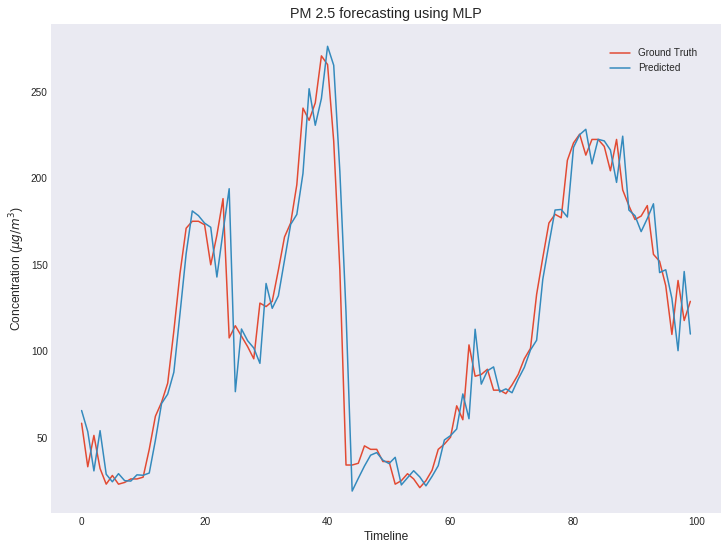
\includegraphics[scale=0.5]{Images/mlp}
	%\centerline{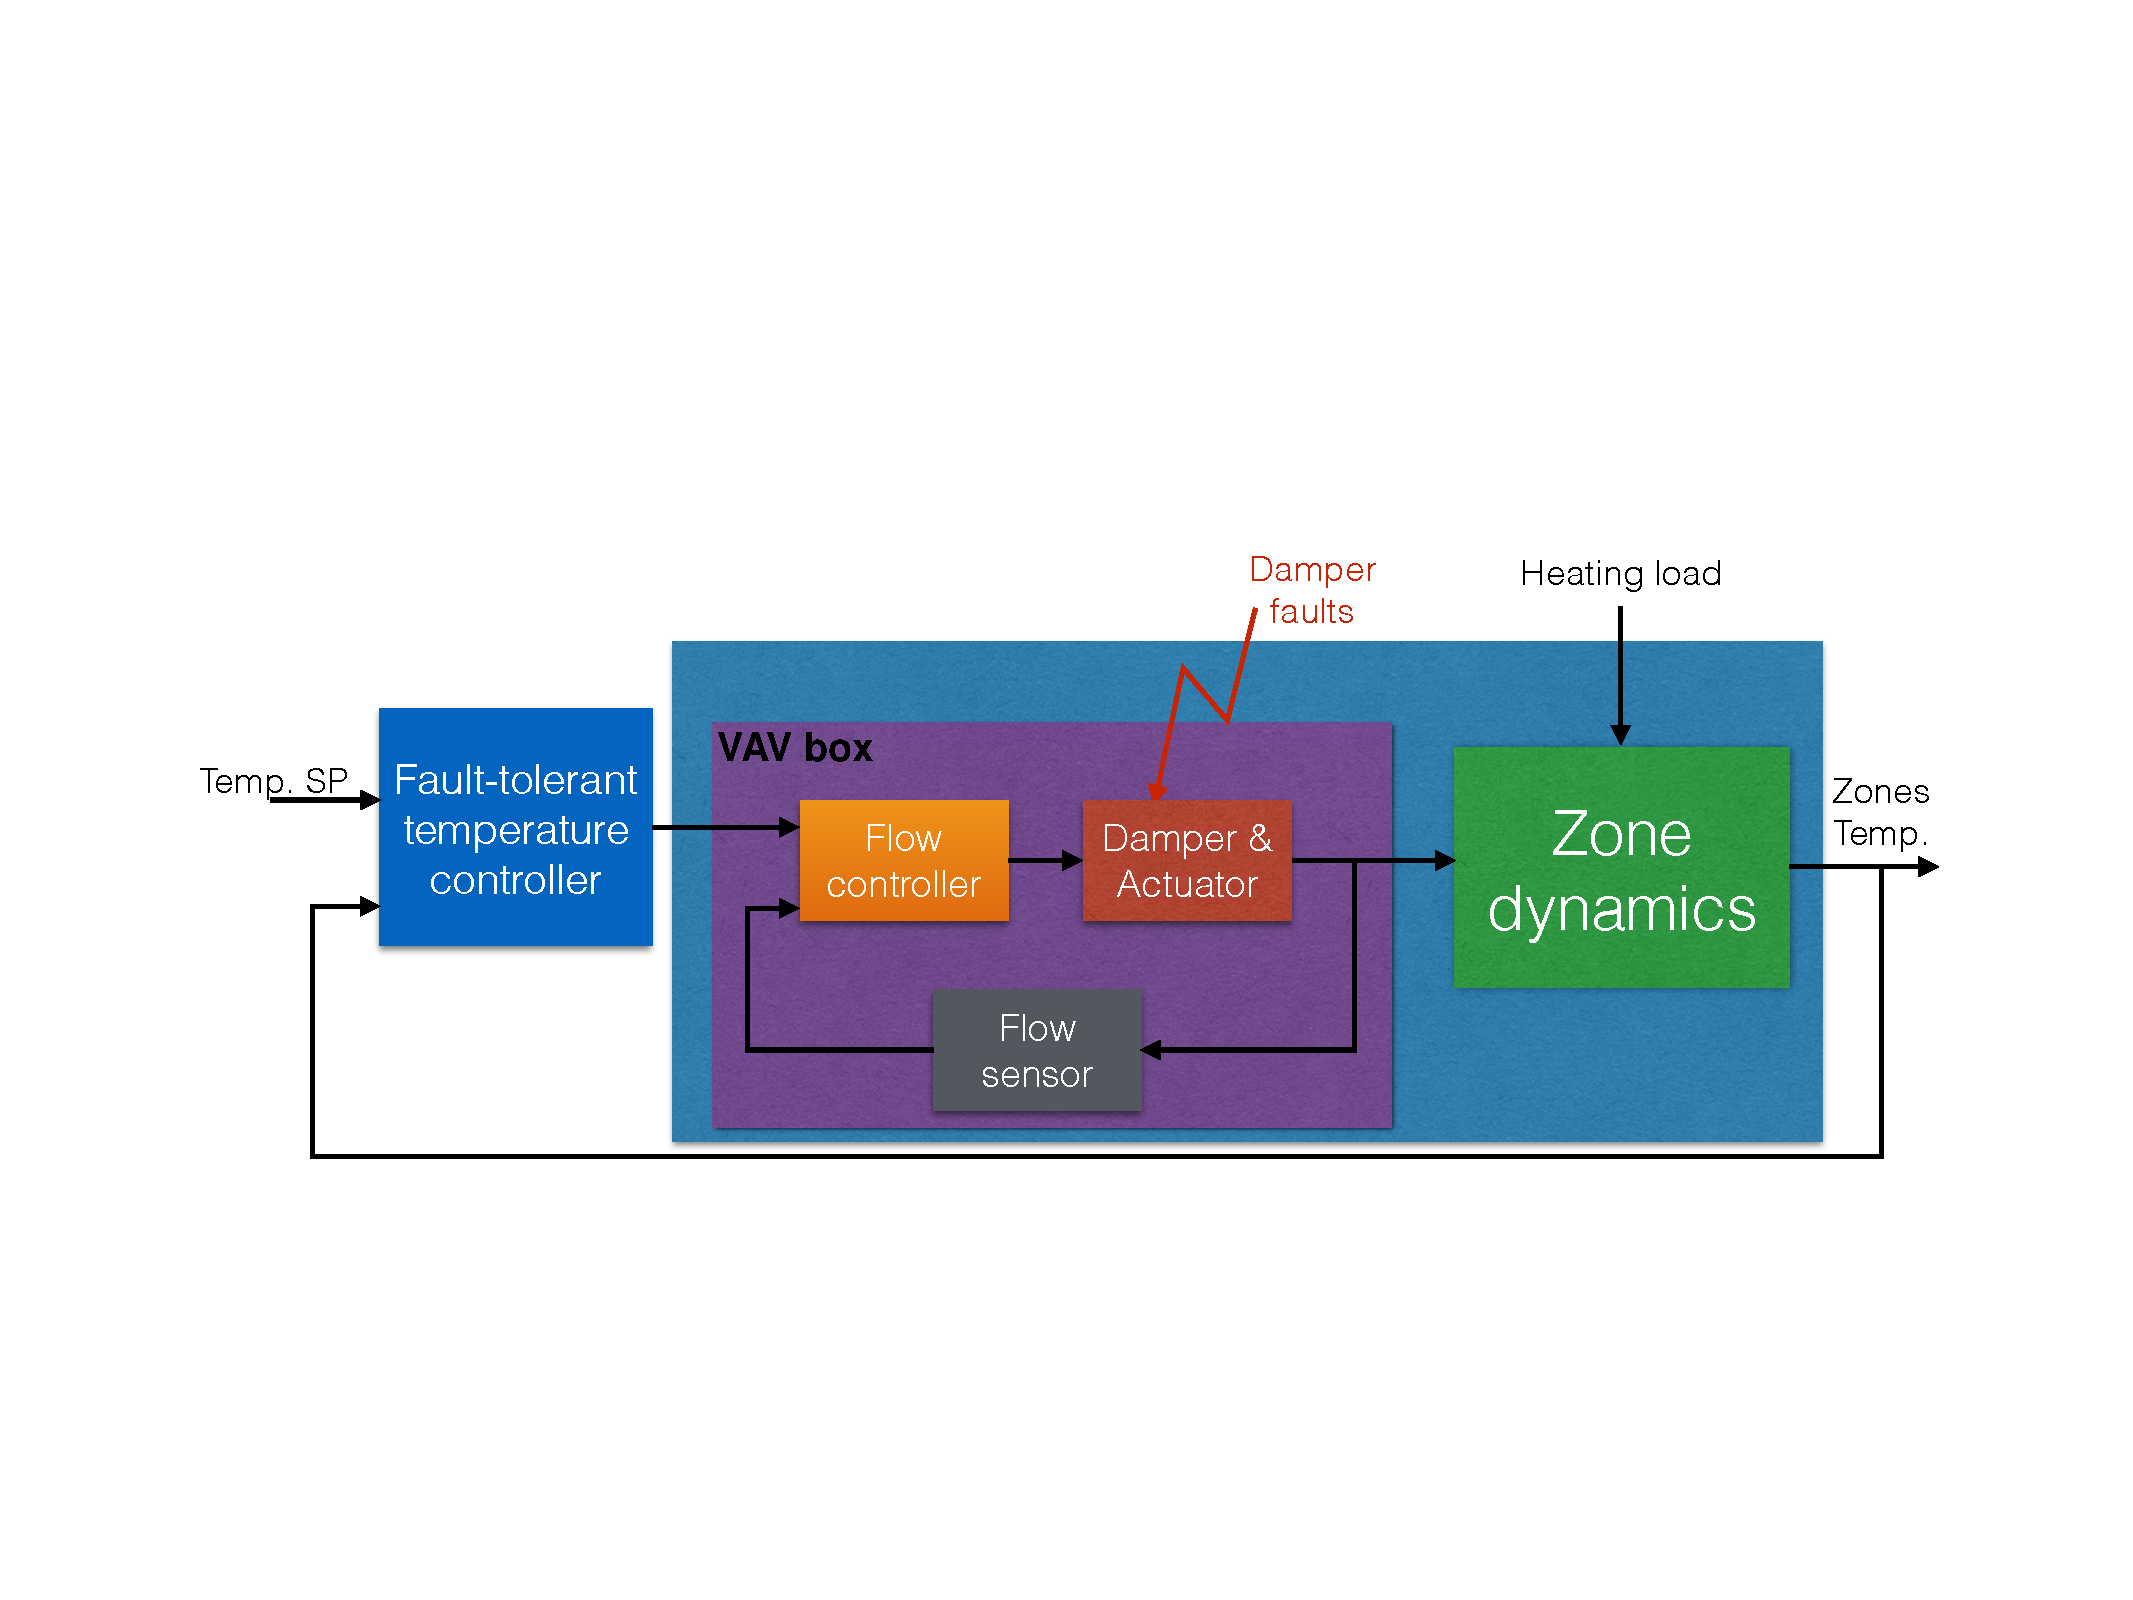
\includegraphics{ftcbuild2.pdf}}
	\caption{Predicted $PM_{2.5}$ concentration.}
	\label{fig}

	\centering
	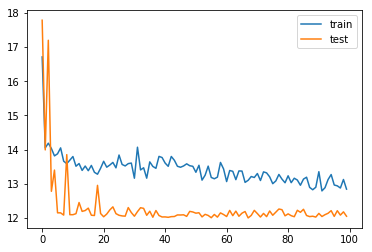
\includegraphics[scale=0.65]{Images/mlp_loss}
	%\centerline{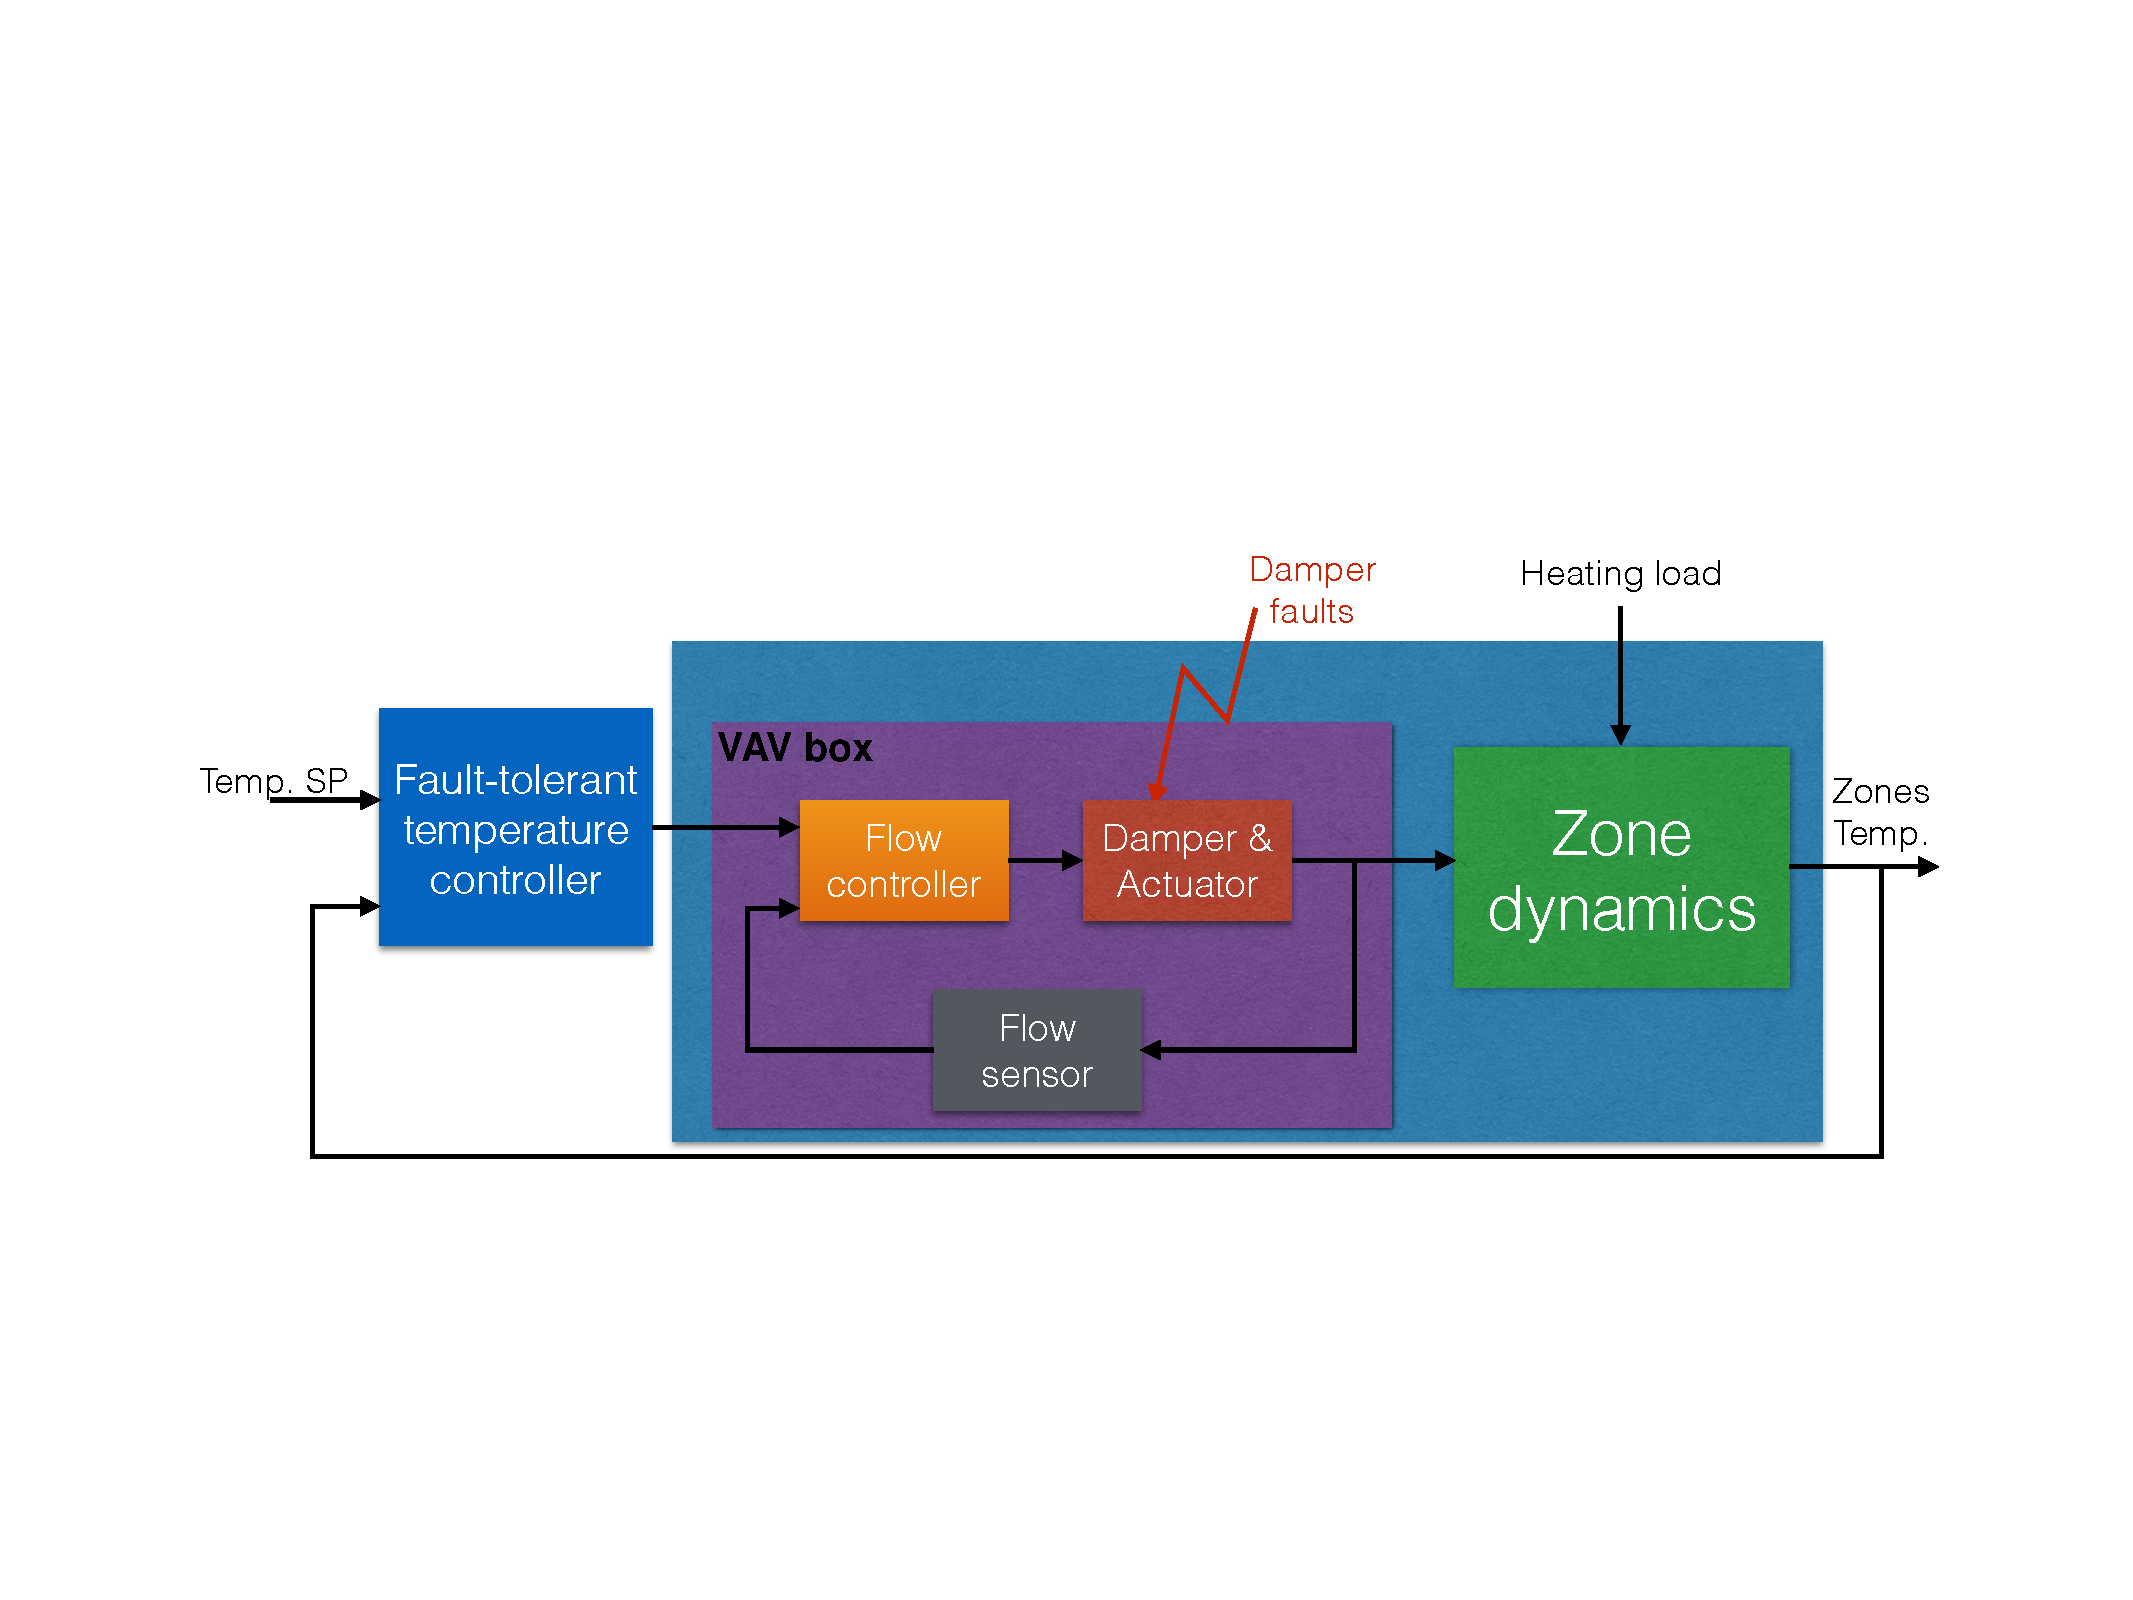
\includegraphics{ftcbuild2.pdf}}
	\caption{Loss curve for MLP.}
	\label{fig}
\end{figure}
Mean Squared Error : 533
\newpage
\subsection{LSTM}
\begin{figure}[htbp]
	\centering
	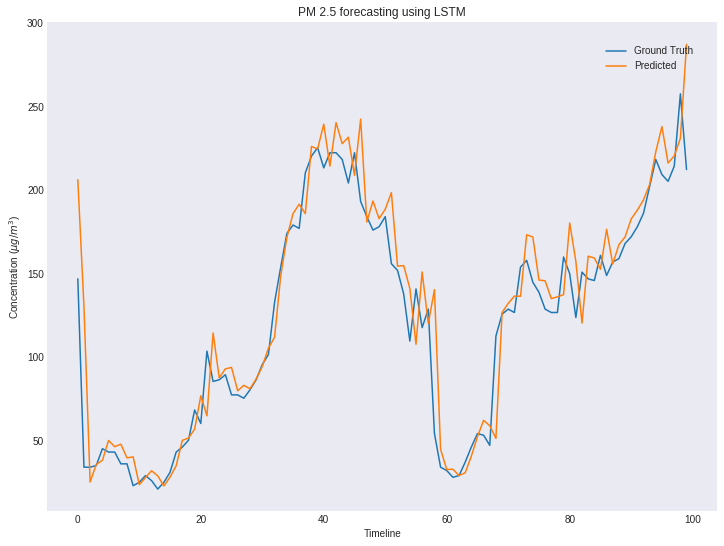
\includegraphics[scale=0.5]{Images/lstm}
	%\centerline{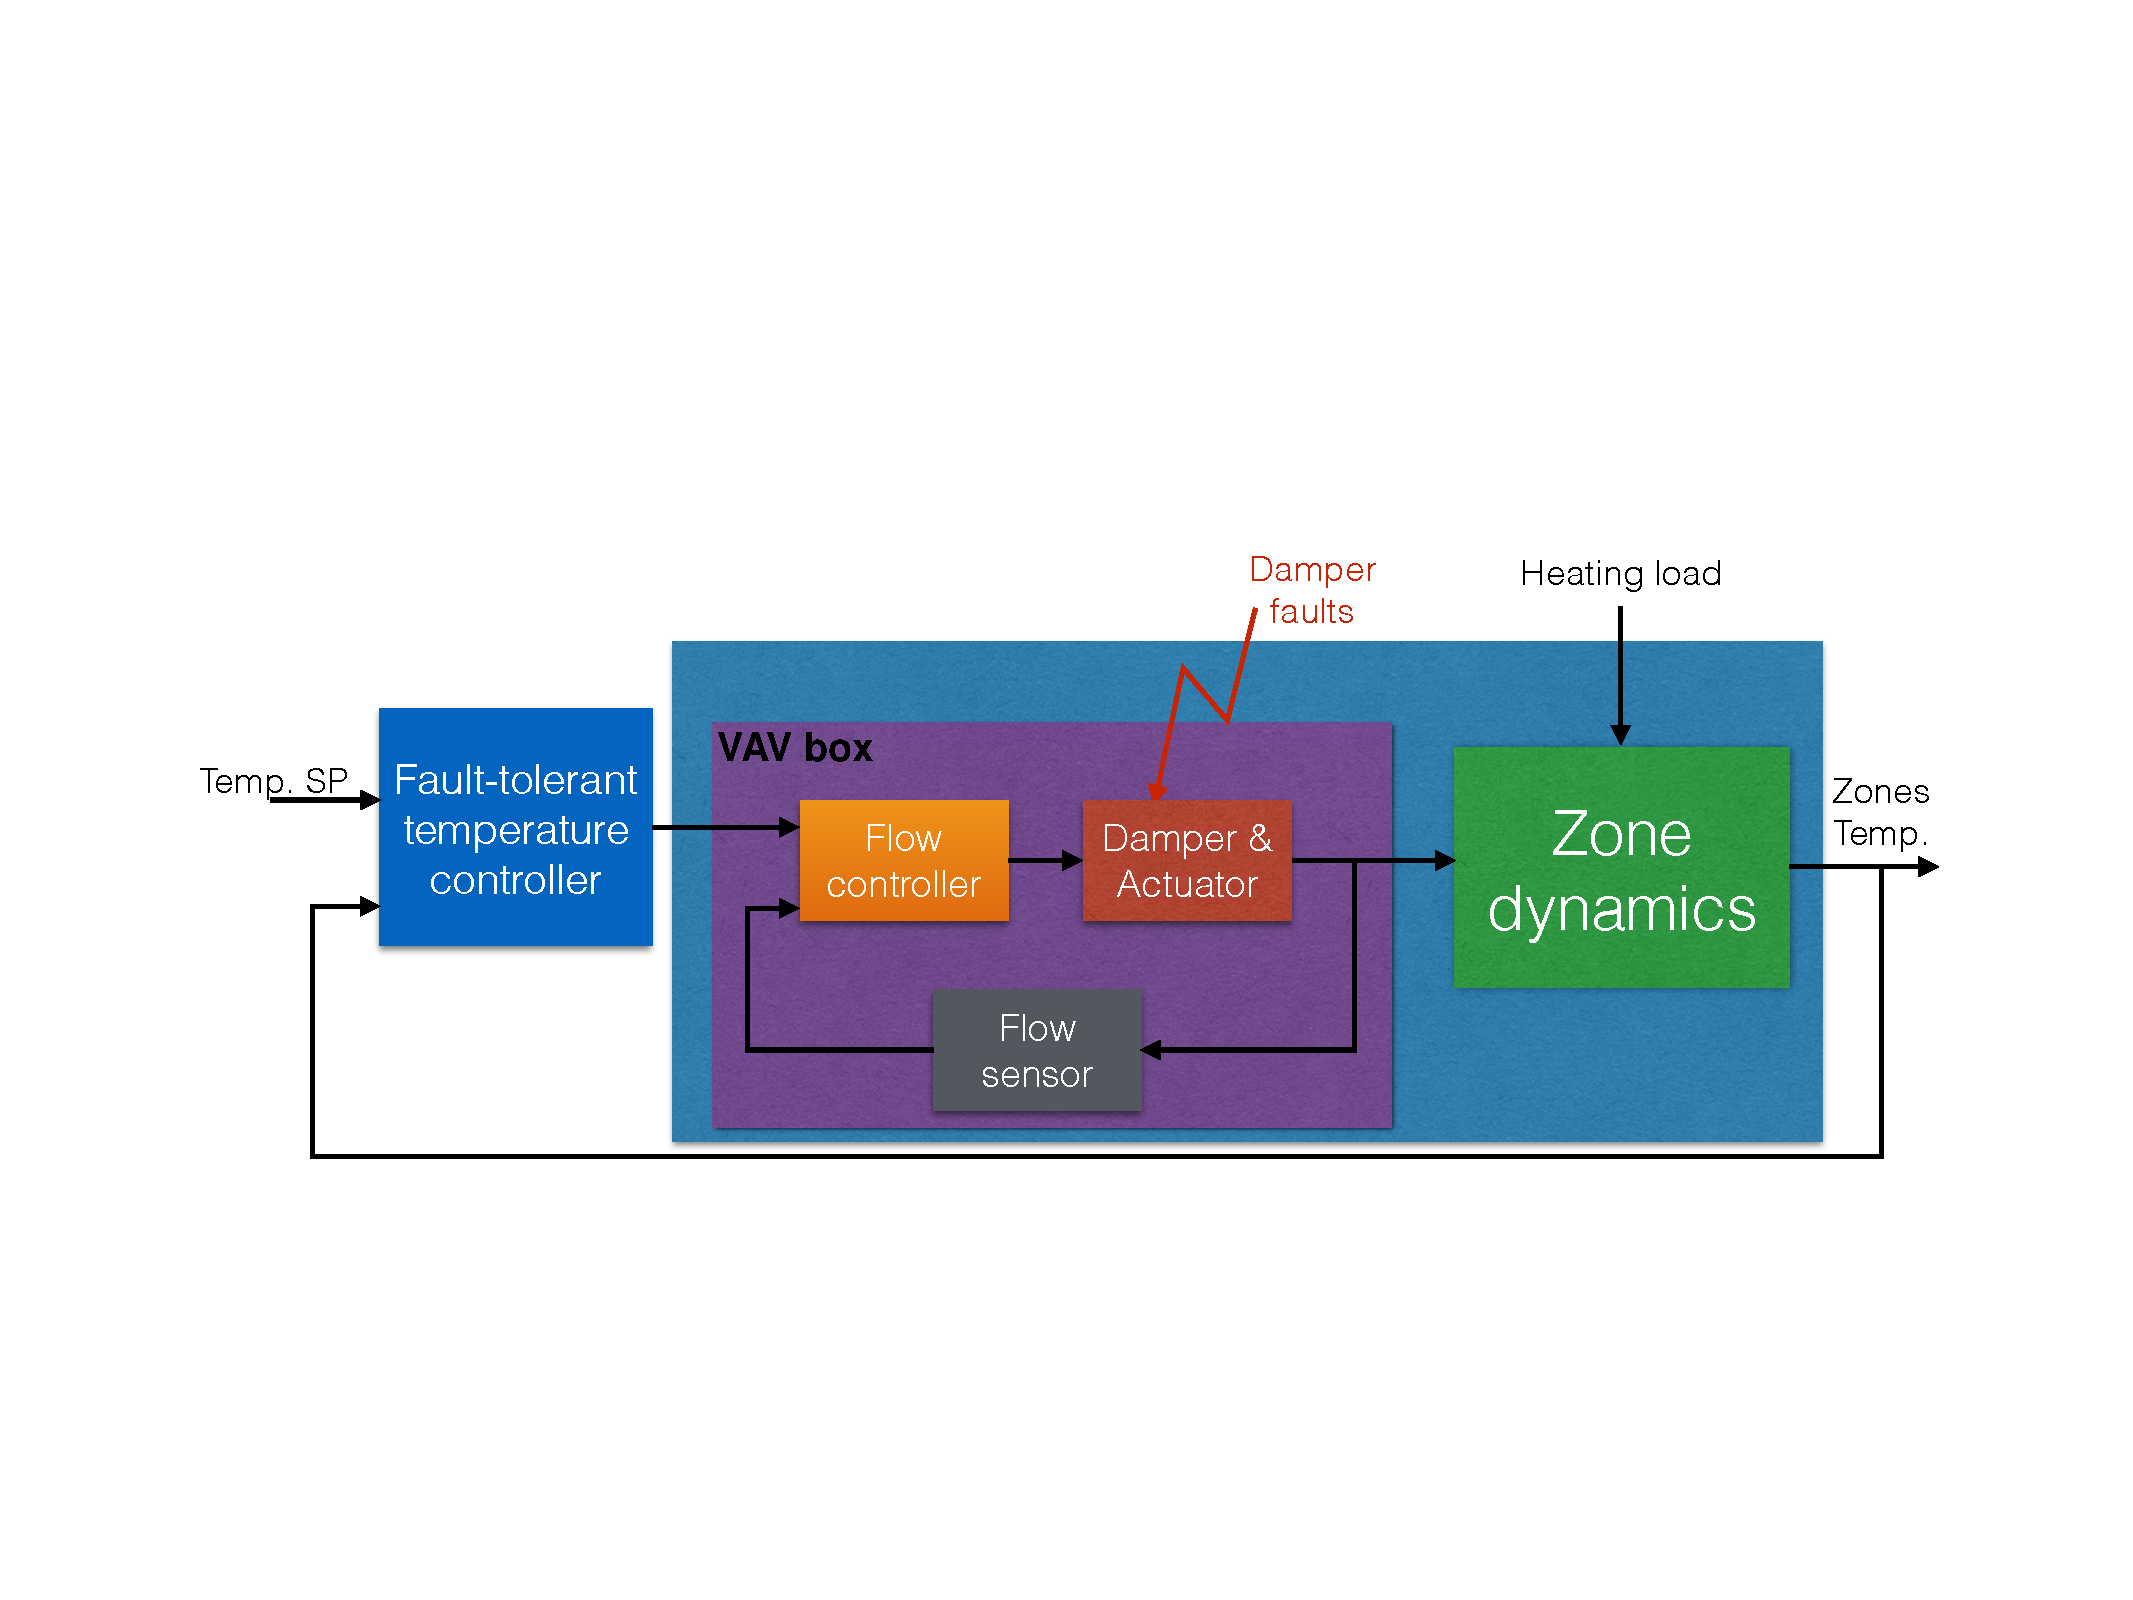
\includegraphics{ftcbuild2.pdf}}
	\caption{Predicted $PM_{2.5}$ concentration.}
	\label{fig}

	\centering
	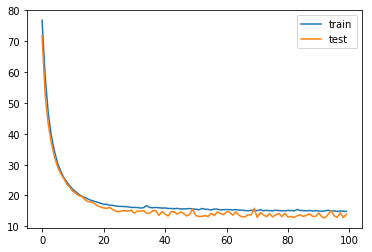
\includegraphics[scale=0.65]{Images/lstm_loss}
	%\centerline{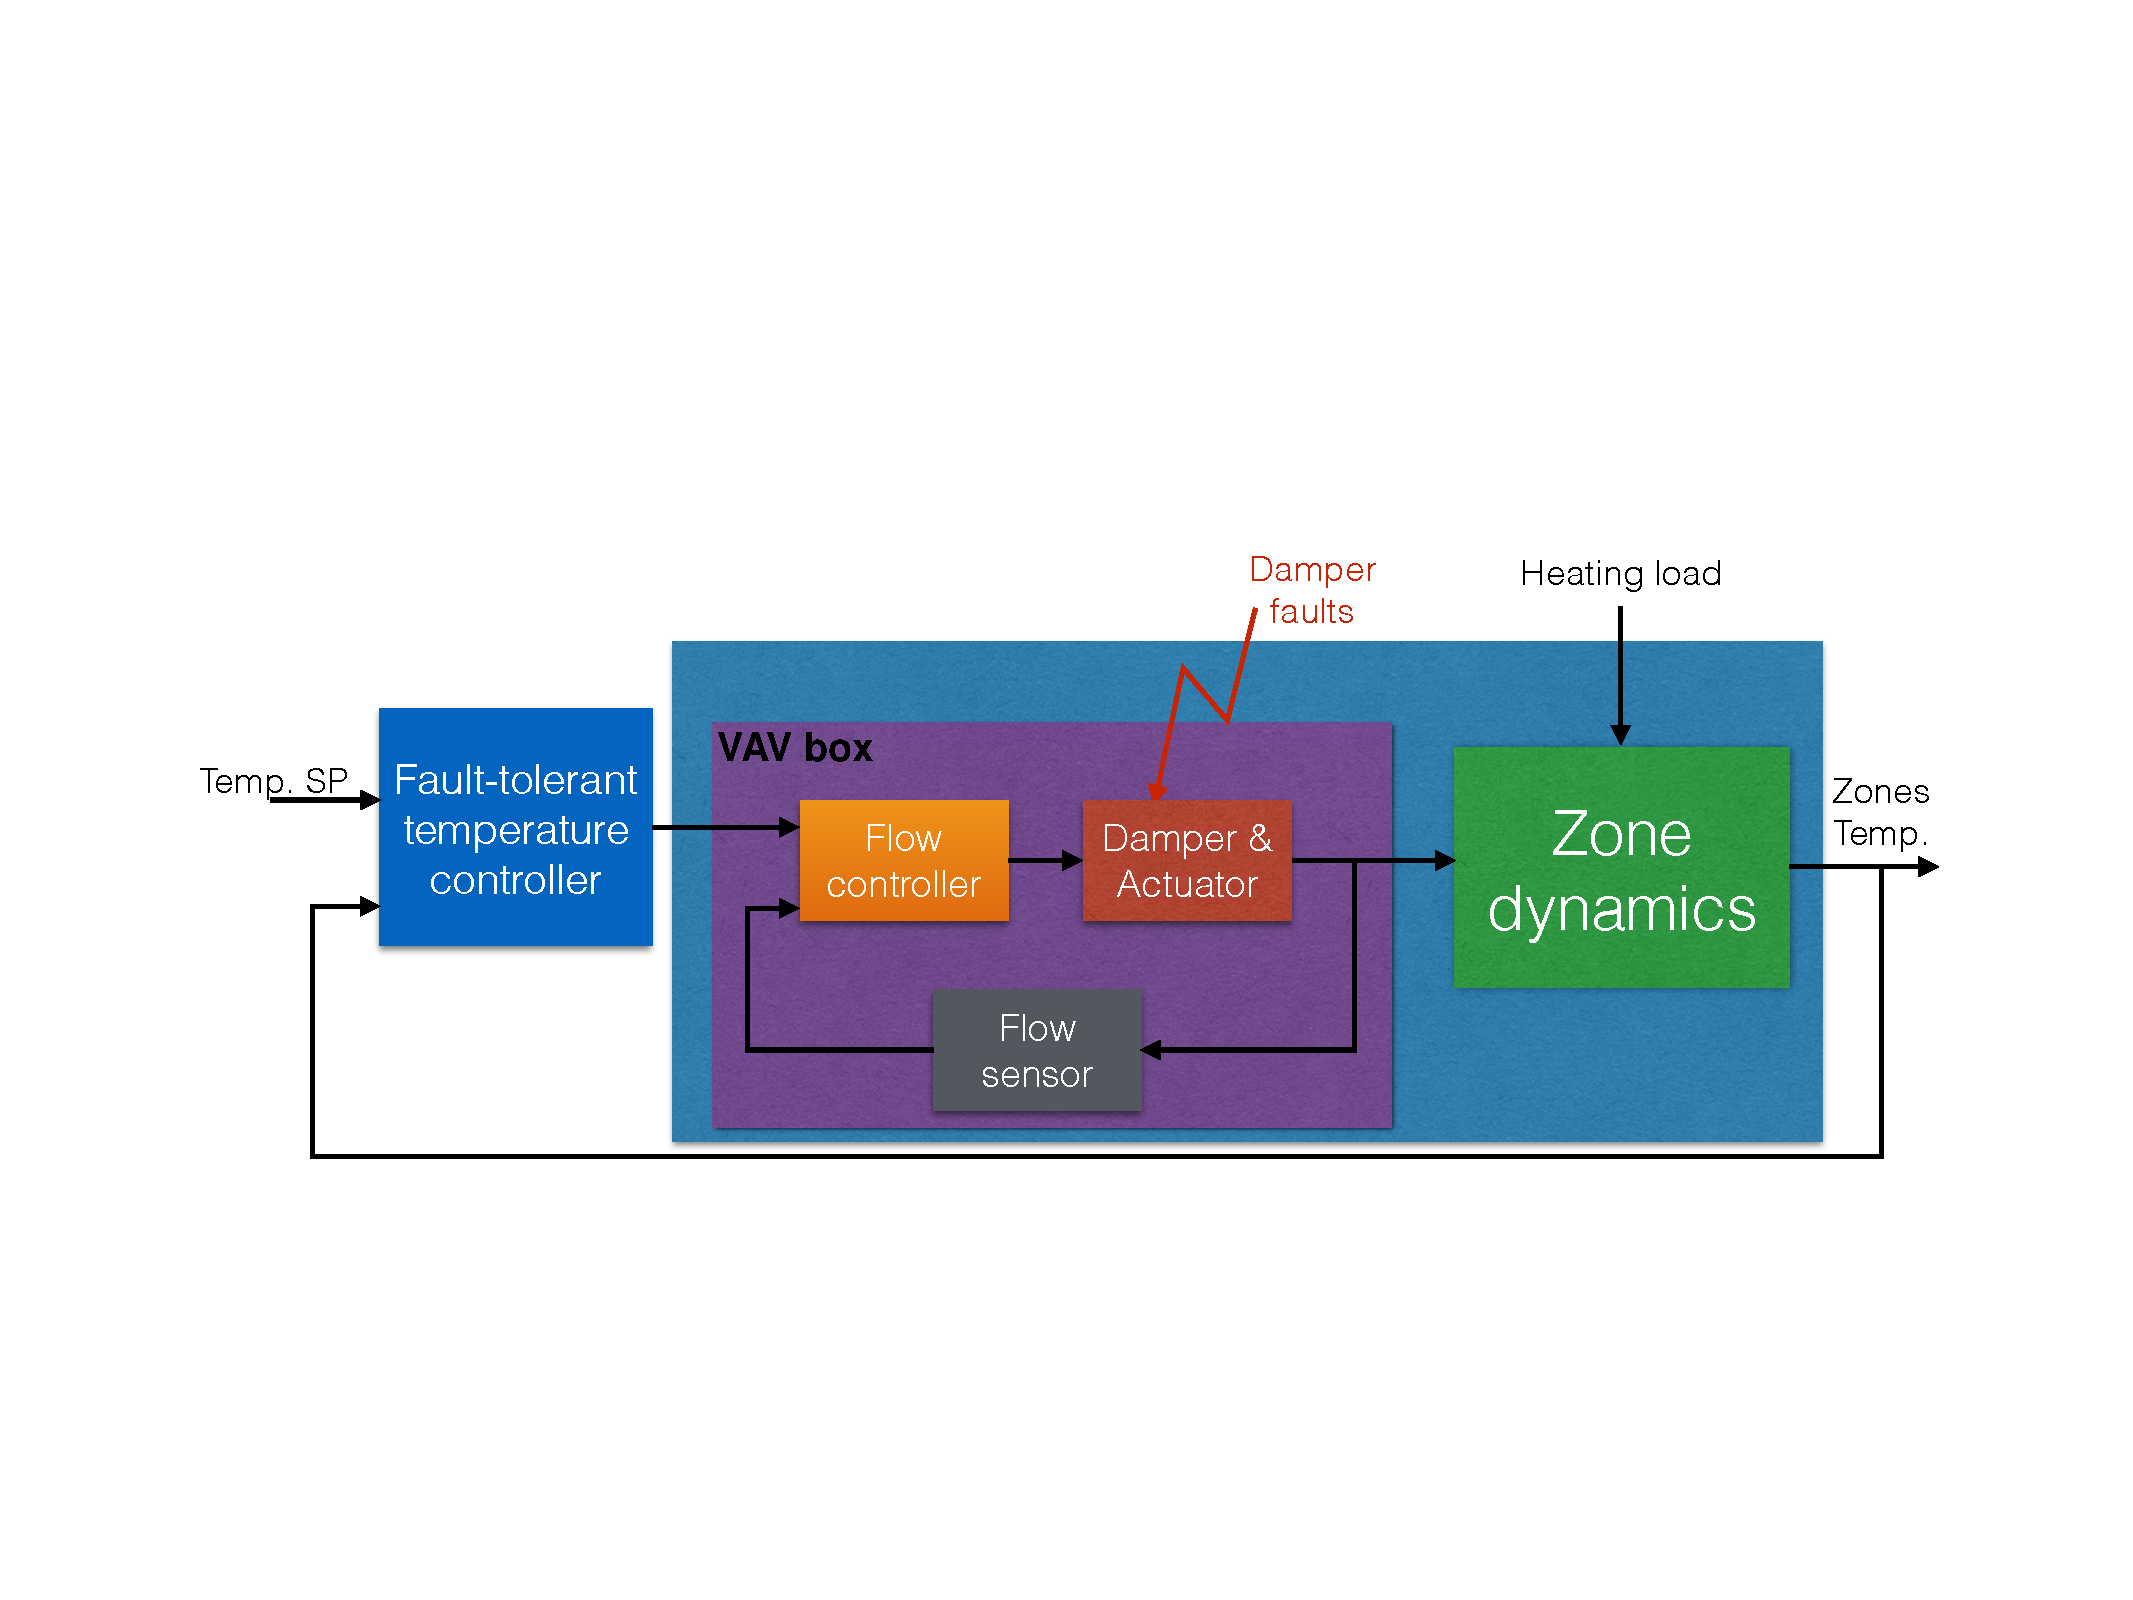
\includegraphics{ftcbuild2.pdf}}
	\caption{Loss curve for LSTM.}
	\label{fig}
\end{figure}	
Mean Squared Error : 640
\newpage
\subsection{CNN}
\begin{figure}[htbp]
	\centering
	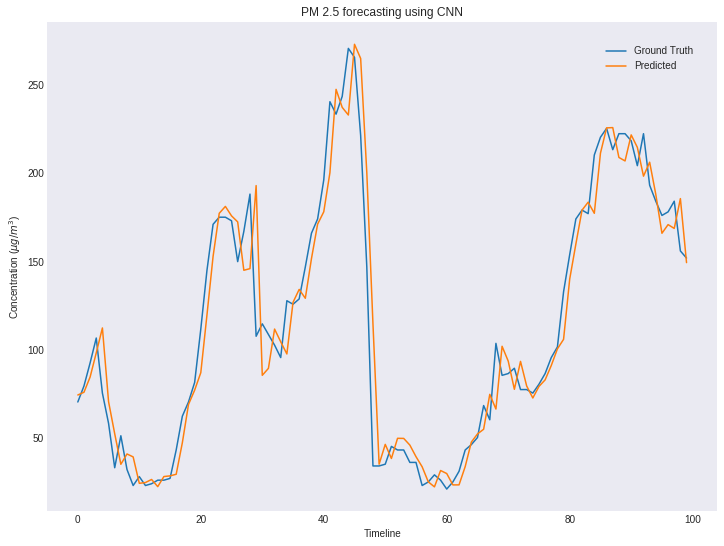
\includegraphics[scale=0.5]{Images/cnn}
	%\centerline{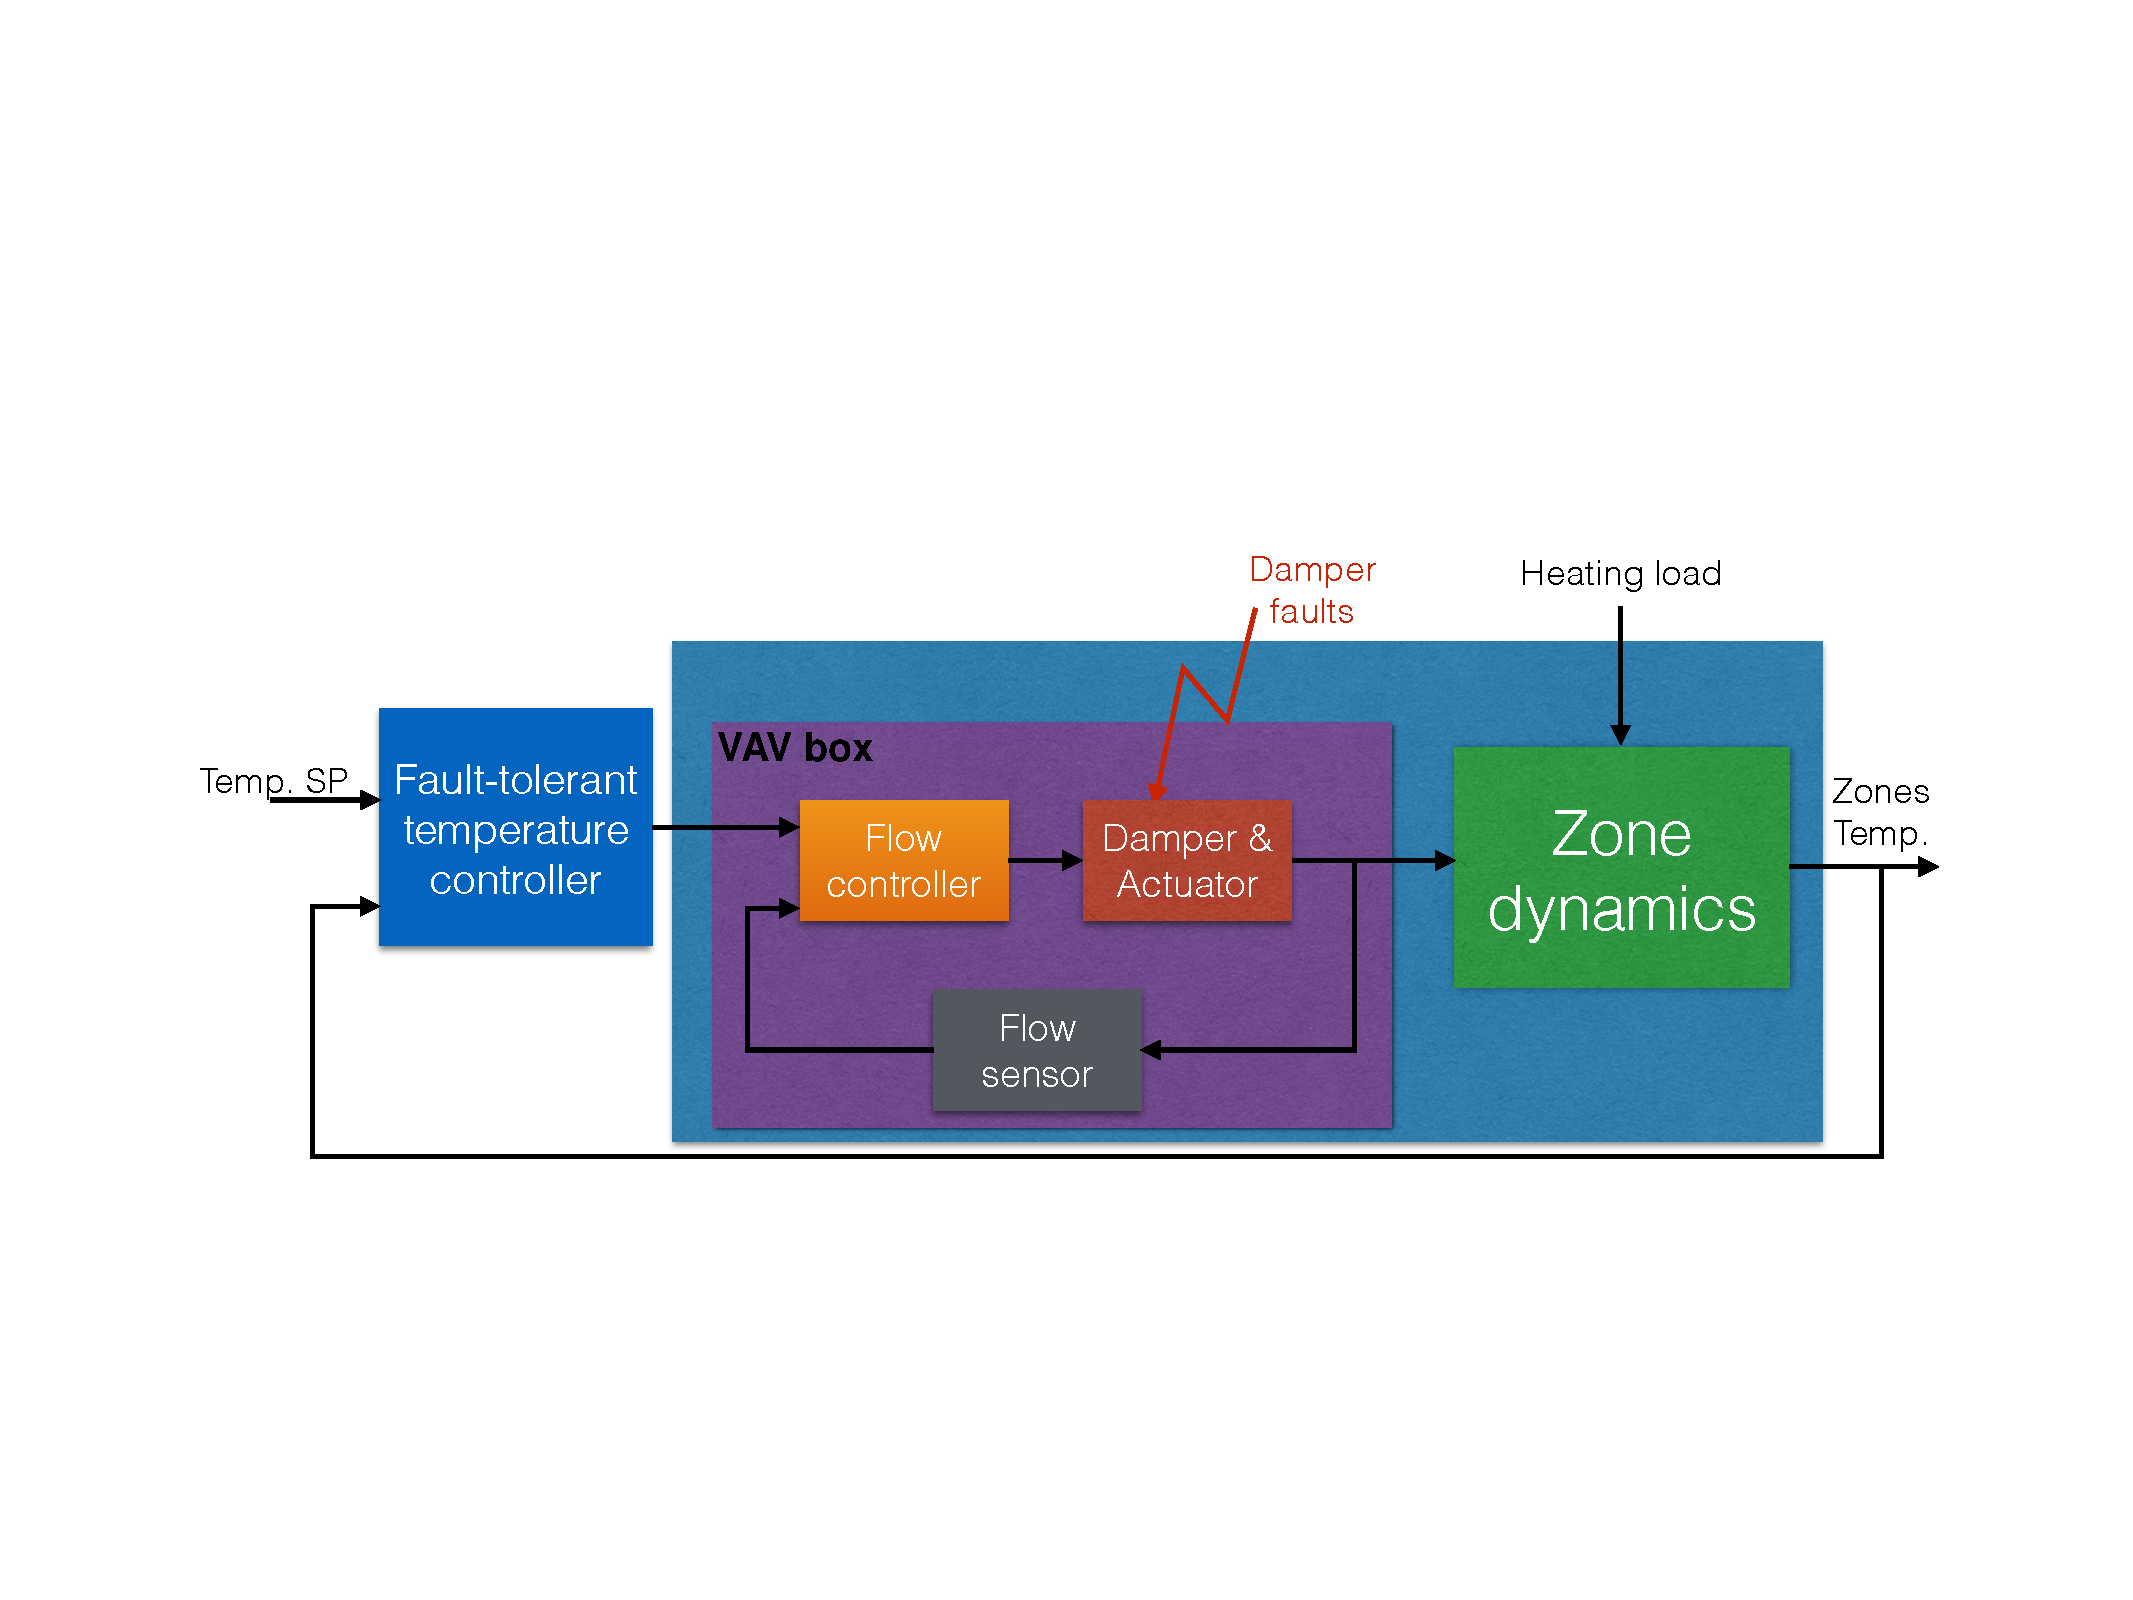
\includegraphics{ftcbuild2.pdf}}
	\caption{Predicted $PM_{2.5}$ concentration.}
	\label{fig}

	\centering
	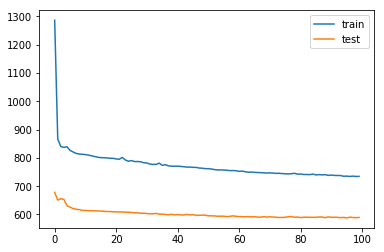
\includegraphics[scale=0.65]{Images/cnn_loss}
	%\centerline{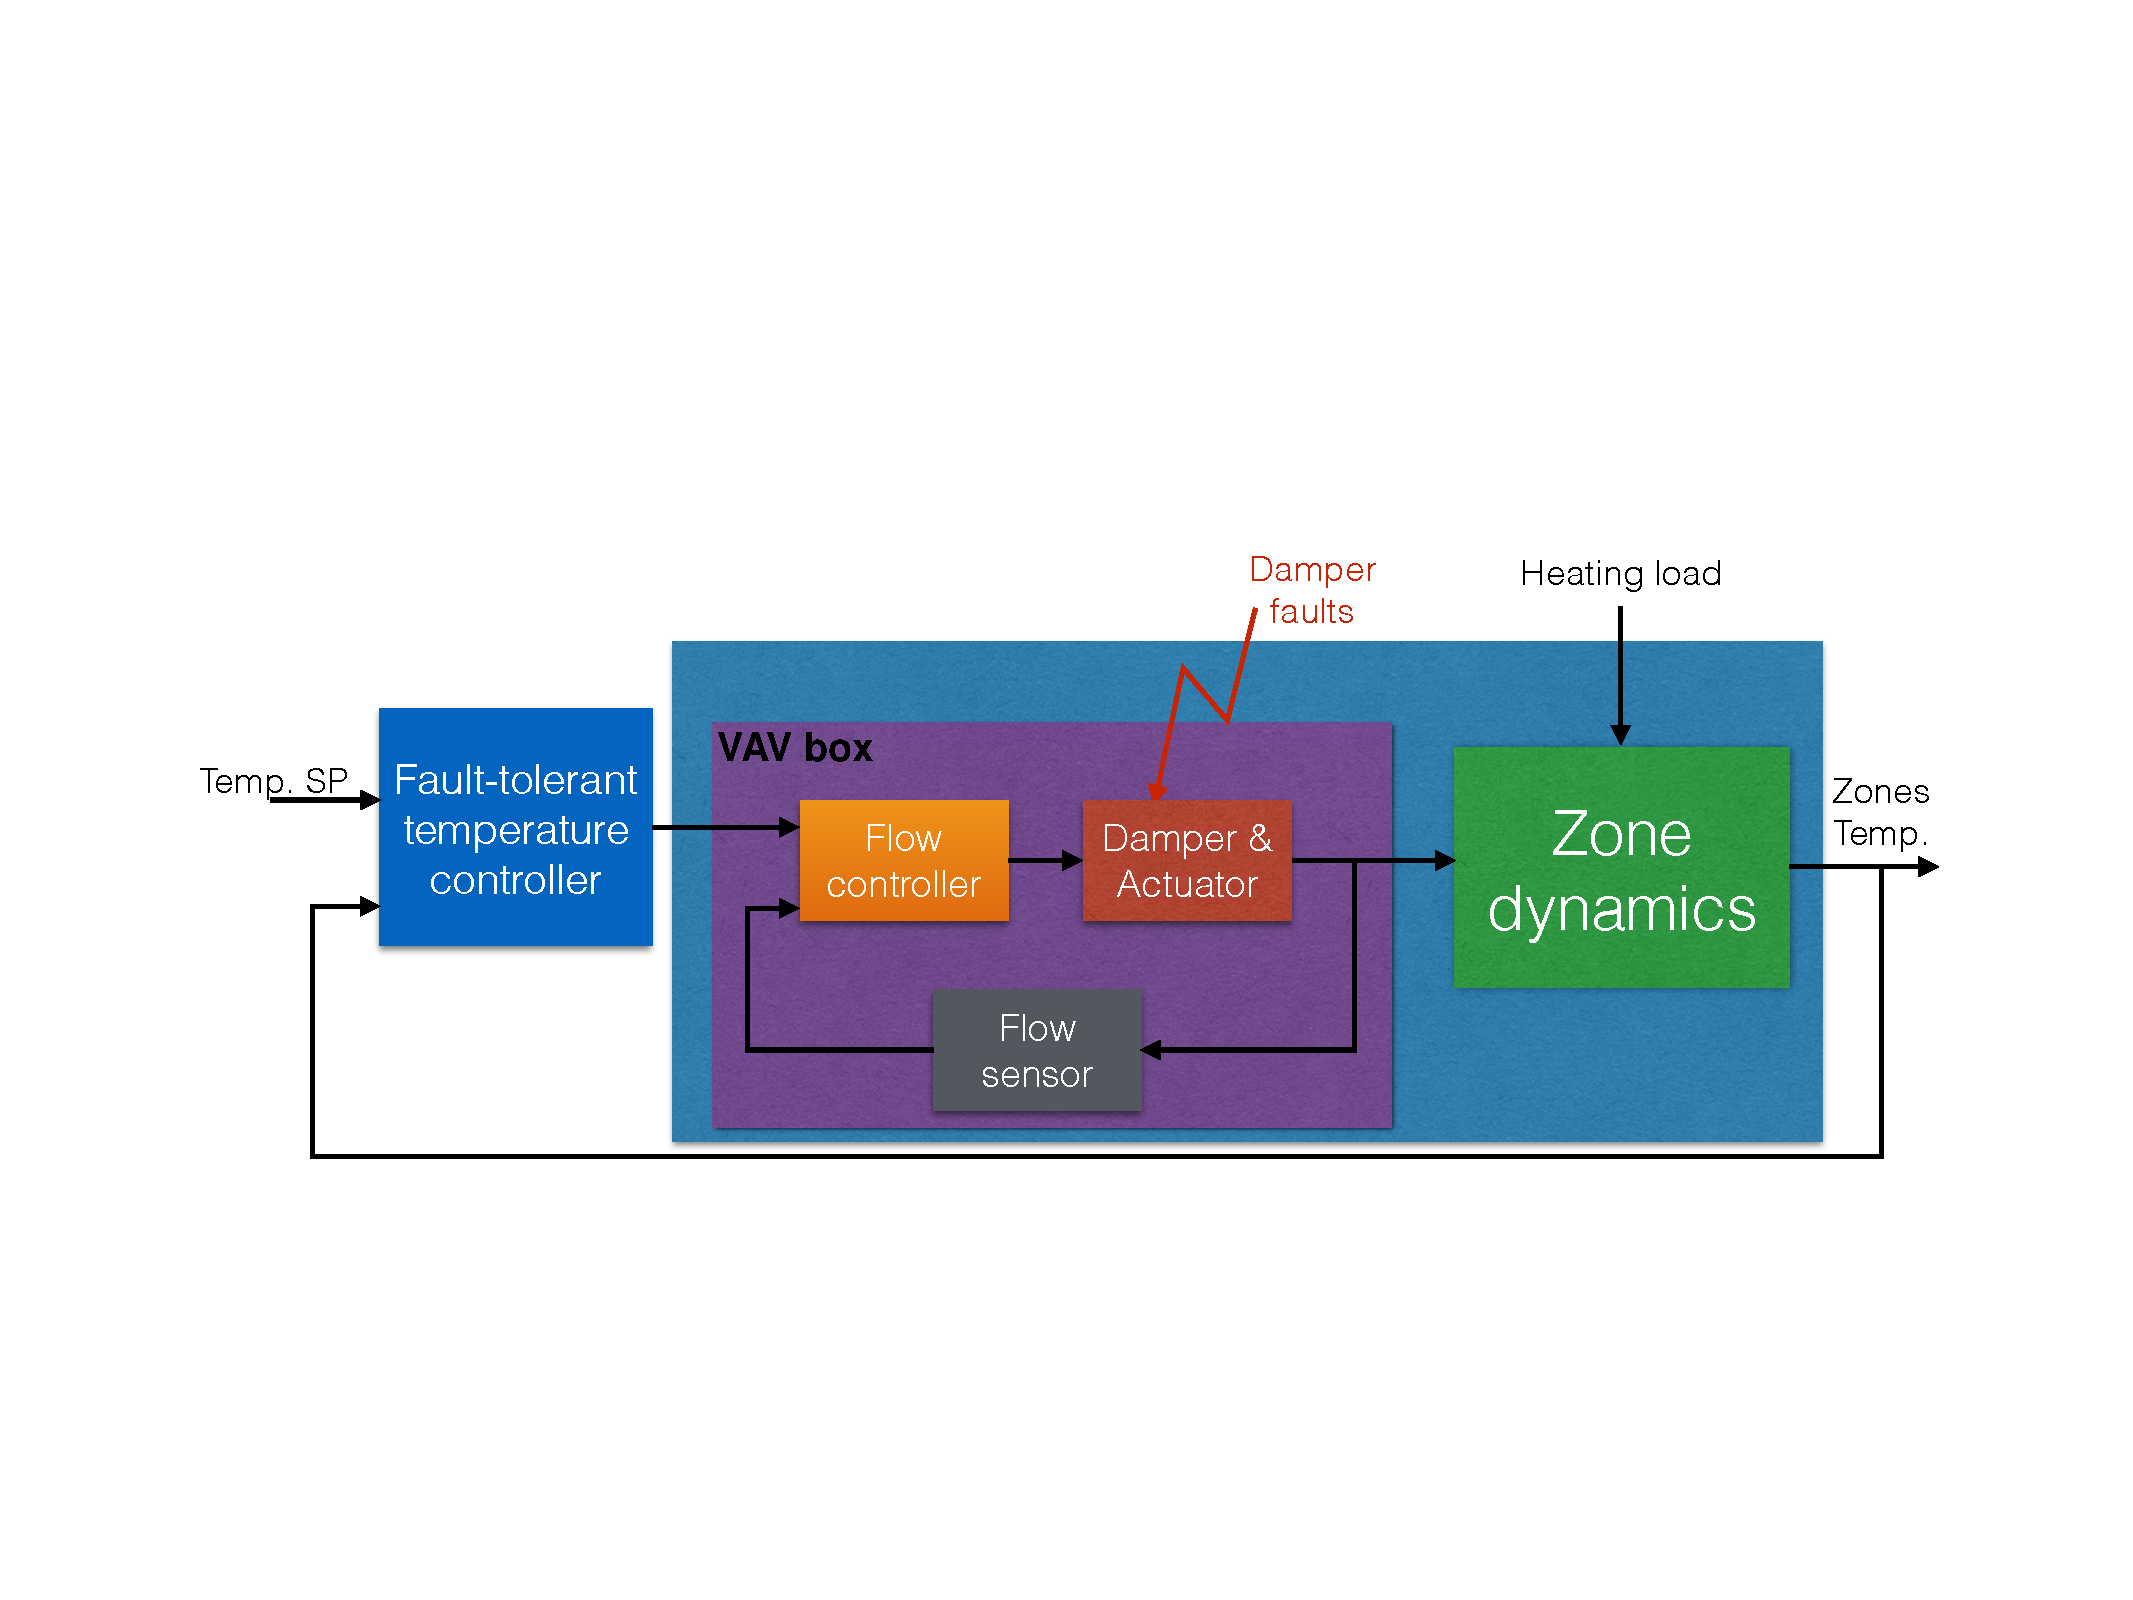
\includegraphics{ftcbuild2.pdf}}
	\caption{Loss curve for CNN.}
	\label{fig}
\end{figure}
Mean Squared Error : 589	
\newpage
\subsection{Grid search for MLP and LSTM}
The $ \mu$ came out to be 0.8185 for the grid search (for MLP).

%\cite{stone2000multiagent}	


\section{Conclusion and Future Work}
Currently we have just tried three models without any fine tuning. We plan on exploring more methodologies for time series forecasting and we finally plan on building an ensemble model with the models which will be performing the best. As an ensemble model would require adding on some hyper-parameters for which we might add a network to make it learn the hyper parameters or we might try attention based learning. \\After exploring all the approaches in the literature, the project will focus on theoretical models of forecasting which involves borrowing ideas from high dimensional probability theory, stochastic processes and stochastic calculus. These approaches will prove benificial in coming up with more domain specific objectives for training deep learning models.

											%CITATION
%\mychapter{2}{Bibliography}                                							%toc

%KEEP BIBLIOGRAPHY IN THESIS.BIB FILE
\bibliographystyle{ieeetr}												%style
\bibliography{report}													%"report" is external file



\end{document}